\chapter{Social and Security Considerations}

\section{Social and security considerations}

The potential of the CubeSats is very high and they might be the future of satellites. Their low cost and the easiness to construct them, compared to large satellites, make them accessible to countries with fewer resources, universities and people in general, making them able to explore the space and to pursue different missions. The assembly of a CubeSat is not very complicated but requires a minimum knowledge about the subject; in other words, now "you've got a user manual, a datasheet and a 3D model that you can download, and you've got an online shop where people can buy their power systems, etc with their credit card" (CITA) \cite{}. 

This project is based on the design of a satellite constellation dedicated to communications relay between LEO satellites and between LEO satellites and the ground. This project is helping to develop the CubeSat industry and its use and it will demonstrate that these small satellites can carry out different missions that were previously done only by large satellites, as for example the communication.

Currently, the constellations of CubeSats dedicated to the communication are in development and the market is not very extensive, this is why this project, and the global coverage that it provides, could have a privileged place in this industry. The main commitment that this project has with the customers is to ensure that they will be able to communicate with any part of the world without problems. 

Another important aspect to consider is that the constellation will provide total privacity  to the costumers, ensuring that they make a correct use of it and avoiding that third people interfering in the communication.

In relation to security, it must ensured the proper functioning of the constellation. To do this, it must be considered three main factors, where CubeSats could be in danger: the launch of the payload, the permanence of the CubeSats in space and the ground stations.

The launch stage is one of the most important, because it is where the mission has more probability to fail. In the next figure can be observed the succes rate of orbital launches in the last 57 years. In 2014, there were a total of 92 unmaned launches and only 4 of them were failed. This indicates that the fail rate is only a 4,34 \%, which is very low. 

\pagebreak

\begin{figure}[h!]
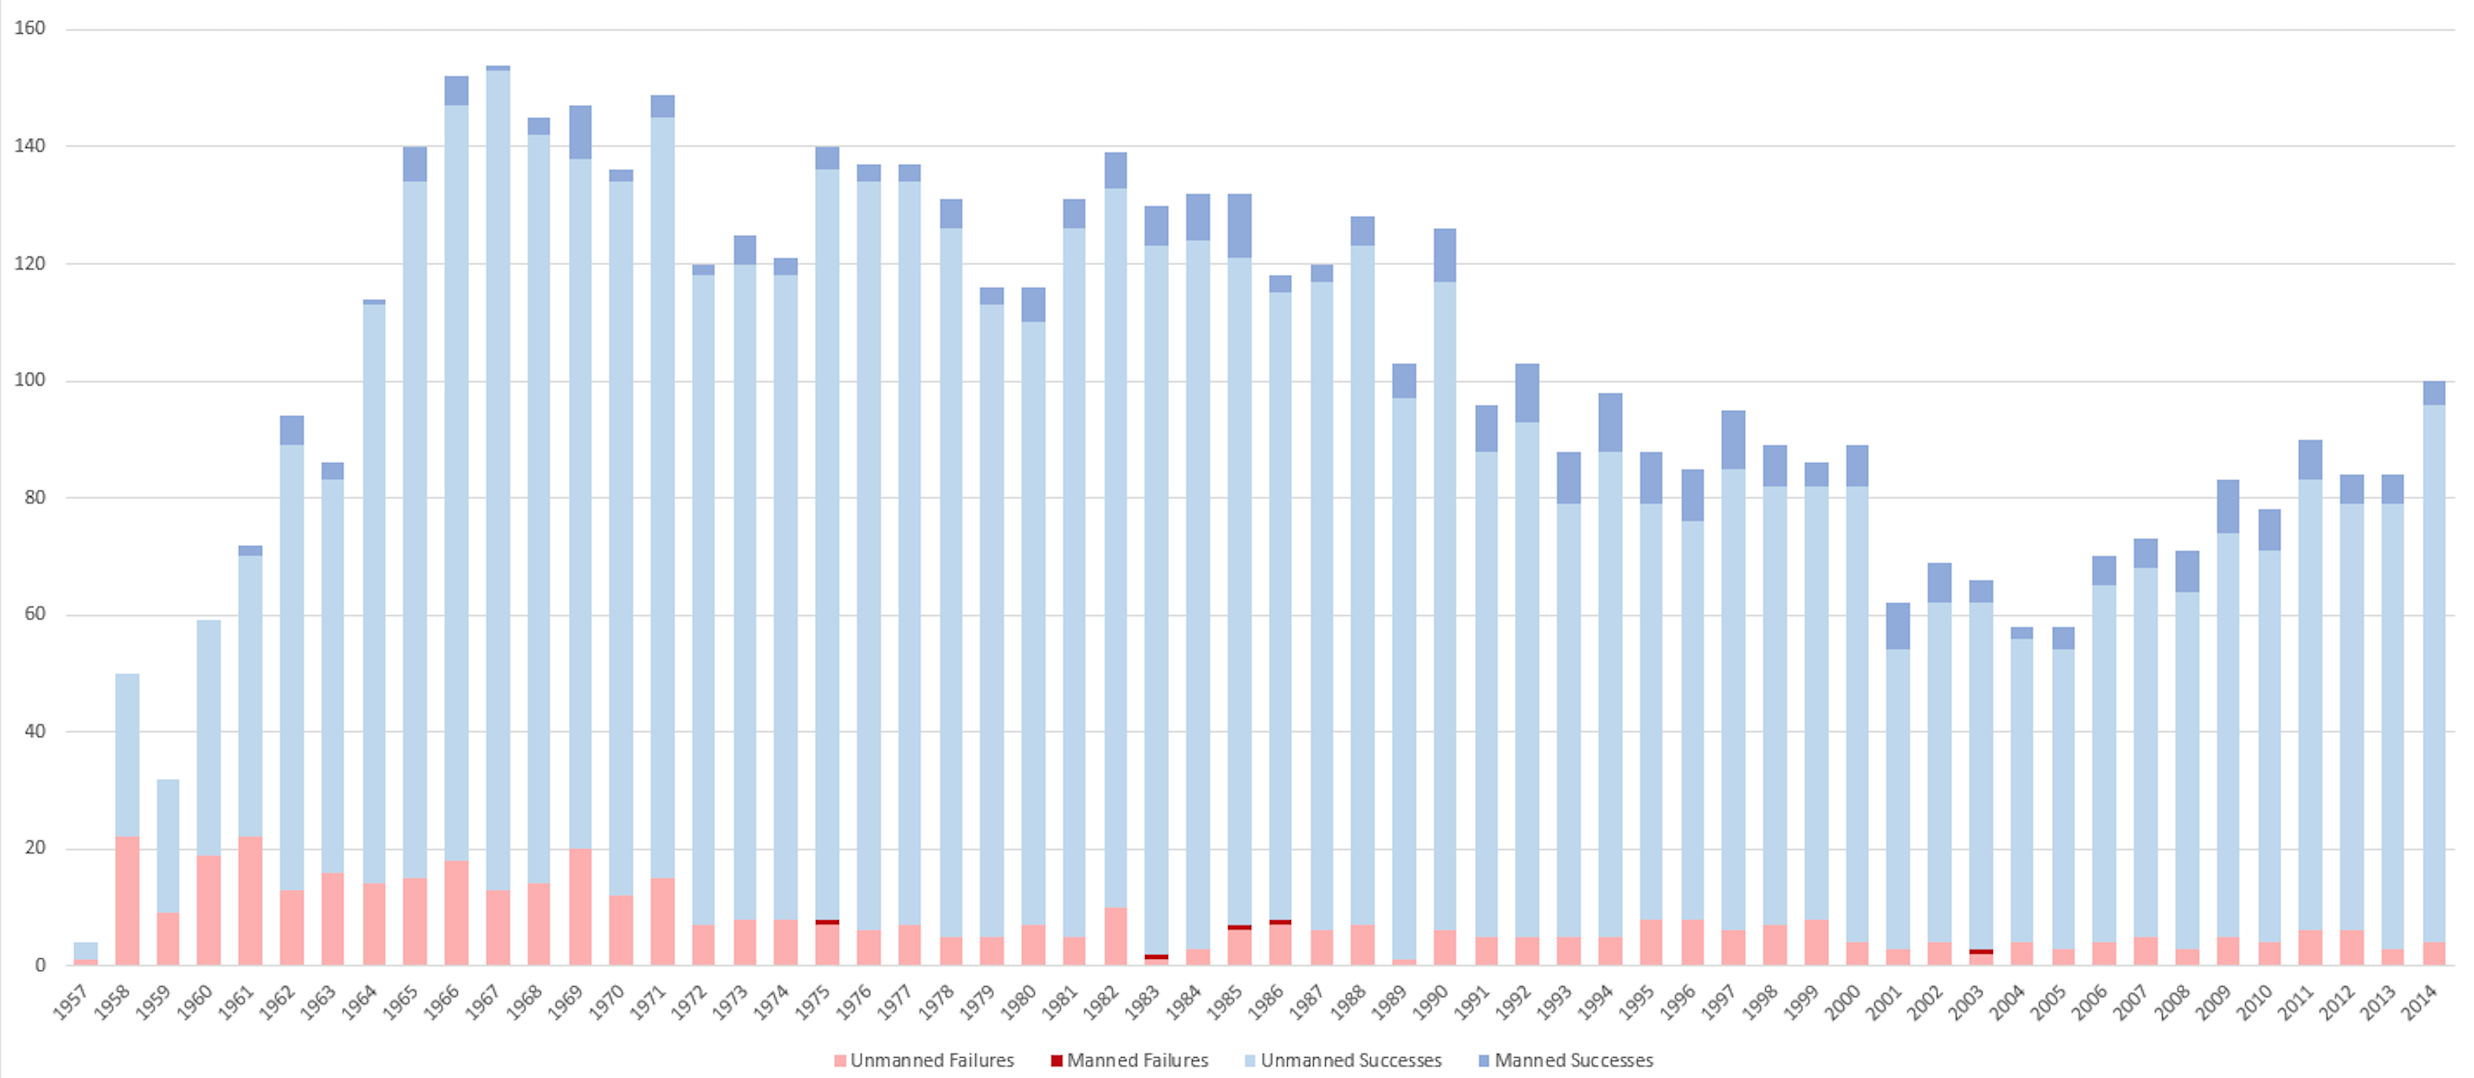
\includegraphics[scale=0.3]{./OrbitalSummary}
\centering
\caption{Orbital Launch Summary by Year}
\end{figure}

\paragraph{}Once the constellation is in orbit, CubeSats can find dangers how colliding with other satellites or with space debris. The distances between most satellites is around hundreds of miles and there is not danger of collision, but the movement of space debris is unpredictable. In order to avoid this space debris, a CubeSat can perform a Debris Avoidance Manoeuvre (DAM). The responsible to control these fragmentation debris is \textit{The United States Space Surveillance Network}. It consists of ground-based radars and optical sensors at 25 sites worldwide and Currently tracks more than 8000 orbiting objects.

Finally, the ground stations are a key element for the correct operation of the constellation and they must prevented from stop working. To do this, each ground station will have its operator, to control the operation of the installation, and a security system, to avoid intrusions.

\section{Legislation}
The legislation concerning activities related to space is the Space Law. Space Law is an international law comprised of international treaties and agreements. Its most important rules are the five international treaties, which have been developed under the supervision of the United Nations. The body that promotes these regulations is the United Nations Office for Outer Space Affairs (UNOOSA).
\newline
\newline
The international law is only applicable to the states that are parties to the treaties. According to the Outer Space Treaty, states are responsible for their national space activities, public or private. For this reason, each state usually adopts its national space regulations.
\newline
\newline
In the case of the Astrea constellation, since the company is based in Spain (a party of the Space Law), the current legislation is the \textit{Real Decreto 278/1995} of 24 February 1995. According to this Royal Decree, the objects launched from Spain or whose launch has been promoted by Spain, should be registered in the \textit{Registro Español de Objetos Espaciales Lanzados al Espacio Ultraterrestre} (Spanish Registry of Objects Launched into Outer Space). The necessary data to register the satellite must be provided to the \textit{Dirección General de Tecnología Industrial del Ministerio de Industria y Energía} (Department of Industrial Technology of the Ministry of Industry and Energy). This department will notificate the registry to the Secretary-General of the United Nations.
\newline
\newline
The registration has to contain the following data:
\begin{enumerate}[label=\alph*)]
\item Name of launching State or States;
\item An appropriate designator of the space object or its registration number;
\item Date and territory or location of launch;
\item Basic orbital parameters, including:
\begin{enumerate}[label=\Roman*)]
\item Nodal period;
\item Inclination;
\item Apogee;
\item Perigee;
\end{enumerate}
\item General function of the space object.
\end{enumerate}
and any other useful information.
For example, in the case of one of the Astrea satellites, the registration will be:
\begin{enumerate}[label=\alph*)]
\item Spain
\item AstreaSAT 1
\item 22 February 2018, 
\item Basic orbital parameters: Low Earth Orbit
\begin{enumerate}[label=\Roman*)]
\item 95,4815 minutes
\item 72 degrees
\item 6.913,0 km
\item 6.913,0 km
\end{enumerate}
\item CubeSat 3U, part of the communications constellation Astrea
\end{enumerate}
